% Asset ID: A21TrigonometryAndModellingTikZ-004
% Purpose: Harmonic maximum/minimum graph
\documentclass[tikz,border=10pt]{standalone}
\usepackage{amsmath}
\usetikzlibrary{arrows.meta}
\begin{document}
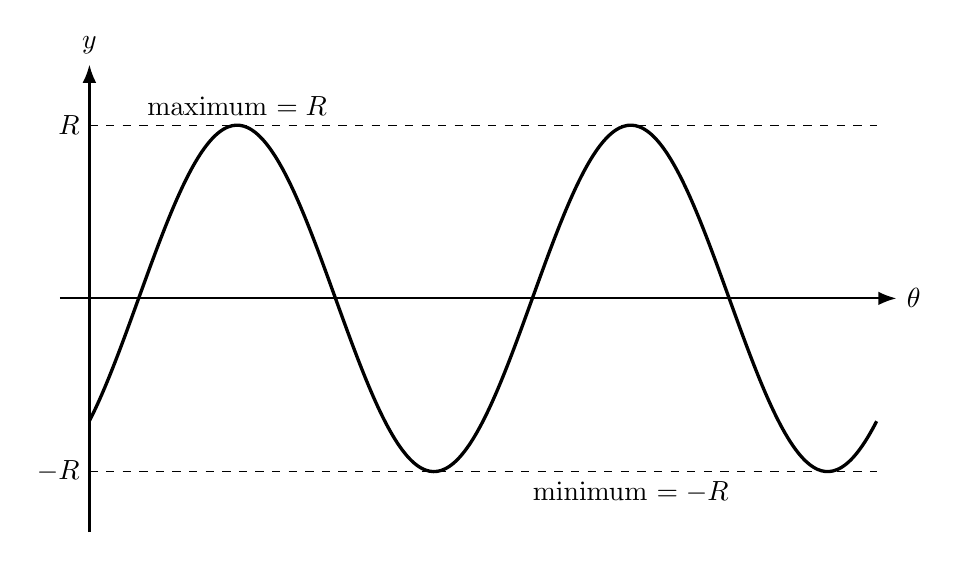
\begin{tikzpicture}[xscale=1.25,yscale=1.1]
\draw[-Latex,thick] (-0.3,0)--(8.2,0) node[right] {\(\theta\)};
\draw[-Latex,thick] (0,-2.7)--(0,2.7) node[above] {\(y\)};
\draw[dashed] (0,2)--(8,2); \draw[dashed] (0,-2)--(8,-2);
\node[left] at (0,2) {\(R\)}; \node[left] at (0,-2) {\(-R\)};
\draw[very thick,domain=0:8,smooth,samples=200] plot (\x,{2*sin((\x*90)-45)});
\node[above] at (1.5,2) {maximum \(=R\)};
\node[below] at (5.5,-2) {minimum \(=-R\)};
\end{tikzpicture}
\end{document}
